\documentclass[trans]{beamer}
\usetheme{CambridgeUS}
\setbeamersize{text margin left=7mm,text margin right=7mm}
\setbeamercovered{transparent}

% Number sets
\newcommand{\N}{\mathbb{N}}
\newcommand{\Z}{\mathbb{Z}}
\newcommand{\Q}{\mathbb{Q}}
\newcommand{\R}{\mathbb{R}}
\newcommand{\C}{\mathbb{C}}
% Math essential packages
\usepackage{latexsym, mathtools}
\usepackage{amsmath, amssymb, amsfonts, amsthm, amsxtra}
\usepackage[nomathsymbols]{polski}

% Diagrams packages
\usepackage{amscd, tikz-cd}

% Package for defining indents and paragraph skips
\usepackage[skip=10pt, indent=0pt]{parskip}

% Package for defining document size, margins etc.
\usepackage[a4paper, left=30mm, right=30mm, top=25mm, bottom=25mm]{geometry}

% Package for handling pictures, images etc.
\usepackage{graphicx, float}

% Package for coloring text
\usepackage{xcolor}

% My favourite font
%\usepackage{XCharter}

% Package for relative font resizing 
\usepackage{relsize}

% Package for creating nice headers and footers
\usepackage{fancyhdr}

% Packages for creating hyperlinks
\usepackage{url}
\usepackage[colorlinks=true,citecolor=blue,urlcolor=blue,linkcolor=blue,pdfpagemode=UseNone]{hyperref}

\title{Wstęp do teorii mocy zbiorów}
\author{Zachariasz Jażdżewski}
\date{21.01.2024}

\begin{document}

%----Proper document------------------------------------------------------------

\frame{\titlepage}

\begin{frame}{Wstęp}
	\visible<1->{Teoria mocy zajmuje się ilością elementów w zbiorze i porównywaniem zbiorów ze względu na ilości ich elementów.}

	\visible<2->{
		Za twórcę teorii mocy, jak i całej teorii mnogości uważa się Georga Cantora.
		\begin{figure}[h]
			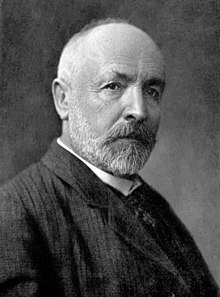
\includegraphics[height=4cm]{cantor.jpg}
		\end{figure}
	}
\end{frame}

\begin{frame}{Równoliczność zbiorów}
	\small
	\begin{columns}
		\begin{column}{0.6\textwidth}
			\visible<1->{
				\begin{block}{Definicja}
					Mówimy, że zbiór $A$ jest równoliczny ze zbiorem $B$, gdy istnieje bijekcja $f$ przekształcająca zbiór $A$ na zbiór $B$. \\
					Zapisujemy jako $A \sim B$.
				\end{block}
			}
			\visible<2->{
				\begin{block}{Przykład}
					Zbiory $A = \{ 1,2,3,4,5 \}$ i $B = \{ 7,8,9,10,11 \}$ są równolicznem, a przykładem funkcji ustalającej równoliczność tych zbiorów może być funkcja 
					\[
						f\colon \{ 1,2,3,4,5 \} \to \{ 7,8,9,10,11 \}
					\]
					taka, że $f(1) = 7, f(2) = 8, f(3) = 9,$ \\ $f(4) = 10, f(5) = 11$ 
				\end{block}
			}
		\end{column}
		\begin{column}{0.4\textwidth}
			\visible<2->{
				\begin{figure}[!ht]
					\centering
					\resizebox{0.9\textwidth}{!}{%
					\begin{circuitikz}
					\tikzstyle{every node}=[font=\LARGE]
					\node [font=\LARGE] at (13,23.75) {1};
					\node [font=\LARGE] at (13,20) {4};
					\node [font=\LARGE] at (13,18.75) {5};
					\node [font=\LARGE] at (13,17.5) {6};
					\node [font=\LARGE] at (13,22.5) {2};
					\node [font=\LARGE] at (13,21.25) {3};
					\node [font=\LARGE] at (18,23.75) {7};
					\node [font=\LARGE] at (18,22.5) {8};
					\node [font=\LARGE] at (18,21.25) {9};
					\node [font=\LARGE] at (18,20) {10};
					\node [font=\LARGE] at (18,18.75) {11};
					\draw  (13,20.75) ellipse (1cm and 3.75cm);
					\draw  (18,20.75) ellipse (1cm and 3.75cm);
					\draw [->, >=Stealth] (14,24) .. controls (15.5,24) and (15.5,24) .. (17,24);
					\draw [->, >=Stealth] (14.25,21.5) .. controls (15.5,21.5) and (15.5,21.5) .. (16.75,21.5);
					\draw [->, >=Stealth] (14.25,20.25) .. controls (15.5,20.25) and (15.5,20.25) .. (16.75,20.25);
					\draw [->, >=Stealth] (14.25,19) .. controls (15.5,19) and (15.5,19) .. (16.75,19);
					\draw [->, >=Stealth] (14.25,22.75) .. controls (15.5,22.75) and (15.5,22.75) .. (16.75,22.75);
					\draw [->, >=Stealth] (14,17.75) .. controls (15.5,17.75) and (15.5,17.75) .. (17,17.75);
					\node [font=\LARGE] at (18,17.5) {12};
					\end{circuitikz}
					}%
				\end{figure}
			}
		\end{column}
	\end{columns}
\end{frame}

\begin{frame}{Podstawowe własności}
	\begin{block}{Twierdzenie}
		Dla dowolnych zbiorów $A, B$ i $C$ zachodzi:
		\begin{enumerate}
			\item<1-> $A \sim A$ 
			\item<2-> $A \sim B \implies B \sim A$ 
			\item<3-> $A \sim B \land B \sim C \implies A \sim C$ 
		\end{enumerate}
	\end{block}
\end{frame}

\begin{frame}{Równoliczność liczb naturalnych z całkowitymi}
	\visible<1->{
		\begin{block}{Twierdzenie}
			Zbiór liczb naturalnych $\N$ jest równoliczny ze zbiorem liczb całkowitych $\Z$.  
		\end{block}
	}
	\visible<2->{
		\begin{block}{Uzasadnienie}
			Równoliczność zbiorów $\Z$ i $\N$ ustala funkcja $f\colon \Z \to \N$ określona wzorem:
			\[
				f(m) = 
				\begin{cases}
					2m & \text{gdy } m \ge 0 \\
					-2m-1 & \text{gdy } m < 0
				\end{cases}
			\]
		\end{block}
	}
\end{frame}

\begin{frame}
	\begin{itemize}
		\item<1-> Łatwo możemy zauważyć, że dla liczb całkowitych nieujemnych funkcja ta zwraca nam zbiór liczb naturalnych parzystych.
		\item<2-> Dla liczb całkowitych ujemnych zaś funkcja zwraca zbiór liczb naturalnych nieparzystych.
		\item<3-> Zatem dla zbioru wszystkich liczb całkowitych funkcja ustala równoliczność ze zbiorem $\N$.
		\item<4-> Jako, że funkcja jest bijekcją, to istnieje również funkcja odwrotna do niej ustalająca równoliczność zbiorów $\N$ i $\Z$. (Dowód, że funkcja $f$ jest bijekcją pomijamy)
	\end{itemize}
\end{frame}

\begin{frame}{Moce zbiorów i porównywanie mocy zbiorów}
	\begin{block}{Definicja}
		Niech $A$ będzie ustalonym zbiorem. Mówimy, że zbiór $A$ jest:
		\begin{enumerate}
			\item<1-> \alert{Skończony}, gdy jest on zbiorem pustym lub jest równoliczny ze
					  zbiorem $\{ 1,2,3,...,n \}$ dla pewnej liczby $n \in \N_+$.
			\item<2-> \alert{Nieskończony}, gdy nie jest on skończony.
			\item<3-> \alert{Przeliczalny}, gdy jest on równoliczny ze zbiorem \\ liczb naturalnych
					  $\N$.
			\item<4-> \alert{Co najwyżej przeliczalny}, gdy jest on skończony lub przeliczalny.
			\item<5-> \alert{Nieprzeliczalny}, gdy nie jest on co najwyżej przeliczalny. 
		\end{enumerate}
	\end{block}
\end{frame}

\begin{frame}{Moc zbioru}
	\begin{block}{Definicja}
		Mocą zbioru $A$ nazywamy cechę przypisaną zbiorowi $A$, oznaczaną przez $|A|$ taką, że:
		\begin{enumerate}
			\item<1-> Mocą zbioru pustego jest $0$ 
				  \[
					  |\varnothing| = 0 
				  \]
			\item<2-> Mocą zbioru skończonego jest liczba jego elementów
				  \[
					  |A| = n, \quad n \in \N_+
				  \]
			\item<3-> Zbiory mają tą samą moc wtedy i tylko wtedy, gdy są one równoliczne
				  \[
				  	  A \sim B \iff |A| = |B|
				  \]
		\end{enumerate}
	\end{block}
\end{frame}

\begin{frame}{Porównywanie mocy zbiorów}
	\visible<1->{Ponieważ moce zbiorów skończonych są liczbami naturalnymi, to można je 
	porównywać. \\}
	\visible<2->{Zdefiniujmy zatem relację do porównywania mocy zbiorów.}
	\visible<3->{
		\begin{block}{Definicja $|A| \le |B|$}
			Mówimy, że \alert{zbiór $A$ ma moc nie większą od zbioru $B$}, jeśli zbiór $A$ jest równoliczny z pewnym podzbiorem zbioru $B$.
		\end{block}
	}
	\visible<4->{
		\begin{block}{Definicja $|A| < |B|$}
			Mówimy, że \alert{zbiór $A$ ma moc mniejszą od zbioru $B$}, gdy 
			\[
				|A| \le |B| \land |A| \ne |B|
			\]
		\end{block}
	}
\end{frame}

\begin{frame}
	\visible<1->{Poznajmy parę elementarnych twierdzeń dotyczących porównywania mocy zbiorów.}
	\visible<2->{
		\begin{block}{Twierdzenie}
			Dla niepustych zbiorów $A$ i $B$ następujące stwierdznia są równoważne
			\begin{enumerate}
				\item $|A| \le |B|$ 
				\item Istnieje iniekcja $f\colon A \overset{1-1}{\longrightarrow} B$ 
				\item Istnieje suriekcja $g\colon B \overset{\text{na}}{\longrightarrow} A$ 
			\end{enumerate}
		\end{block}
	}
	\visible<3->{
		\begin{block}{Własności}
			Dla dowolnych zbiorów $A, B$ i $C$ mamy:
			\begin{enumerate}
				\item<4-> $|A| \le |A|$ 
				\item<5-> $|A| \le |B| \ \land\  |B| \le |C| \implies |A| \le |C|$ 
				\item<6-> $|A| \le |B| \ \land\  |B| \le |A| \implies |A| = |B|$ 
				\item<7-> $|A| \le |B| \ \lor\ |B| \le |A|$ 
			\end{enumerate}
		\end{block}
	}
\end{frame}

\begin{frame}{Nieprzeliczalność liczb rzeczywistych na odcinku $(0,1)$}
	\visible<1->{
		\begin{block}{Twierdzenie}
			Odcinek otwarty $(0,1)$ nie jest przeliczalny
		\end{block}
	}
	\visible<2->{
		Udowodnimy to twierdzenie używając metody przekątniowej Cantora.
	}
	\visible<3->{
		Zauważmy, że każda liczba rzeczywista $x \in (0,1)$ ma swoje rozwinięcie dziesiętne.
	}
	\visible<4->{
		Jeśli jest ono skończone, to uzupełniamy rozwinięcie o nieskończoną ilość zer.
	}
\end{frame}

\begin{frame}
	Ponumerujmy wszystkie liczby rzeczywiste $x \in (0,1)$ liczbami naturalnymi ustawiając je w nieskończony ciąg indeksowany po $\N$:
	\visible<2->{
		\begin{align*}
			\N & \quad x \in (0,1) \\
			1 & \quad 0.\ 1\ 2\ 6\ 8\ 7\ 4\ 1\ 5\ 2\ 7\ ...\\
			2 & \quad 0.\ 6\ 5\ 8\ 7\ 9\ 2\ 1\ 7\ 8\ 6\ ...\\
			3 & \quad 0.\ 2\ 4\ 2\ 3\ 8\ 1\ 2\ 0\ 4\ 5\ ...\\
			4 & \quad 0.\ 8\ 2\ 3\ 0\ 4\ 2\ 6\ 5\ 8\ 4\ ...\\
			5 & \quad 0.\ 3\ 7\ 9\ 8\ 5\ 0\ 0\ 1\ 2\ 8\ ...\\
			6 & \quad 0.\ 9\ 3\ 2\ 7\ 8\ 9\ 4\ 7\ 8\ 9\ ...\\
			7 & \quad 0.\ 5\ 8\ 9\ 6\ 7\ 8\ 9\ 1\ 2\ 0\ ...\\
			8 & \quad 0.\ 7\ 2\ 3\ 6\ 2\ 4\ 9\ 1\ 9\ 2\ ...\\
			9 & \quad ...\\
		\end{align*}
	}
\end{frame}

\begin{frame}
	\small
	\begin{columns}
		\begin{column}{0.4\textwidth}
			Skonstruujmy teraz liczbę rzeczywistą $a \in (0,1)$. Stworzymy ją w taki sposób:
			\begin{enumerate}
				\item<1-> Weźmiemy pierwszą cyfrę po przecinku o indeksie $1$ i dodamy $1$ 
				\item<2-> Weźmiemy drugą cyfrę po przecinku o indeksie $2$ i dodamy $1$ 
				\item<3-> Weźmiemy trzecią cyfrę po przecinku o indeksie $3$ i dodamy $1$ 
			\end{enumerate}
			\visible<4->{i tak dalej... \\}
			\visible<4->{Jeżeli cyfra po przecinku to $9$, to zamieniamy ją na $0$.}
		\end{column}
		\begin{column}{0.4\textwidth}
			\begin{align*}
				\N & \quad x \in (0,1) \\
				\visible<1->{1 & \quad 0.\ \textbf{\alert{1}}\ 2\ 6\ 8\ 7\ 4\ 1\ 5\ 2\ 7\ ...\\}
				\visible<2->{2 & \quad 0.\ 6\ \textbf{\alert{5}}\ 8\ 7\ 9\ 2\ 1\ 7\ 8\ 6\ ...\\}
				\visible<3->{3 & \quad 0.\ 2\ 4\ \textbf{\alert{2}}\ 3\ 8\ 1\ 2\ 0\ 4\ 5\ ...\\}
				\visible<4->{4 & \quad 0.\ 8\ 2\ 3\ \textbf{\alert{0}}\ 4\ 2\ 6\ 5\ 8\ 4\ ...\\}
				\visible<4->{5 & \quad 0.\ 3\ 7\ 9\ 8\ \textbf{\alert{5}}\ 0\ 0\ 1\ 2\ 8\ ...\\}
				\visible<4->{6 & \quad 0.\ 9\ 3\ 2\ 7\ 8\ \textbf{\alert{9}}\ 4\ 7\ 8\ 9\ ...\\}
				\visible<4->{7 & \quad 0.\ 5\ 8\ 9\ 6\ 7\ 8\ \textbf{\alert{9}}\ 1\ 2\ 0\ ...\\}
				\visible<4->{8 & \quad 0.\ 7\ 2\ 3\ 6\ 2\ 4\ 9\ \textbf{\alert{1}}\ 9\ 2\ ...\\}
				\visible<4->{9 & \quad ...\\}
				  & \\
				a & \quad 0.\ \alert{
						\visible<1->{2\ }
						\visible<2->{6\ }
						\visible<3->{3\ }
						\visible<4->{1\ 6\ 0\ 0\ 2}...
					}
			\end{align*}
		\end{column}
	\end{columns}
\end{frame}

\begin{frame}{Wniosek}
	W efekcie otrzymaliśmy liczbę $a \in (0,1)$, która różni się od każdej liczby w naszym ciągu o conajmniej jedną cyfrę, zatem liczba $a$ nie występuje w ciągu, wbrew temu, że ciąg zawierał wszystkie liczby rzeczywiste. 
	\visible<2->{
		\begin{block}{Wniosek}
			Otrzymana sprzeczność pokazuje, że zbiory liczb naturalnych i rzeczywistych z przedziału 
			$(0,1)$ nie są równoliczne.
		\end{block}
	}
\end{frame}

\begin{frame}{Przykłady innych zbiorów przeliczalnych, co najwyżej przeliczalnych i nieprzeliczalnych}
	\begin{itemize}
		\item<1-> Zbiór liczb rzeczywistych $\R$ jest nieprzeliczalny. 
			      ($\R \nsim \N$)
		\item<2-> Zbiór $\N \times \N$ jest przeliczalny. 
			      ($\N \times \N \ \sim\  \N$)
		\item<3-> Zbiór liczb wymiernych $\Q$ jest przeliczalny. 
			      ($\Q \sim \N$)
		\item<4-> Zbiór liczb niewymiernych $\R \setminus \Q$ jest zbiorem nieprzeliczalnym. 
			      ($\R \setminus \Q \ \nsim\ \N$) 
		\item<5-> Żaden zbiór nie jest równoliczny ze zbiorem wszystkich swoich podzbiorów. 
			      ($A \nsim \mathcal{P}(A)$) 
		\item<6-> Każdy nieprzeliczalny podzbiór zbioru liczb rzeczywistych $\R$ jest równoliczny
				  ze zbiorem $\R$.		
	\end{itemize}
\end{frame}

\begin{frame}{Źródła}
	\begin{enumerate}
		\item Jerzy Topp, \textit{Wstęp do matematyki}, Wydawnictwo Uniwersytetu Gdańskiego, Gdańsk 2015
		\item Joanna Cyman, \textit{Wykłady z przedmiotu "Wstęp do logiki i teorii mnogości"}, Politechnika Gdańska, Gdańsk 2023/2024
	\end{enumerate}
\end{frame}

%-------------------------------------------------------------------------------

\end{document}
